%!TEX root = /Users/ego/Boulot/TKZ/tkz-graph/doc-fr/TKZdoc-gr-main.tex

% $Id$
\section{Les labels}
%<–––––––––––––––––––––––––––––––––––––––––––––––––––––––––––––––––––––––––>

%<–––––––––––––––––––––––––––––––––––––––––––––––––––––––––––––––––––––––––>
%                             Options sur les labels
%<–––––––––––––––––––––––––––––––––––––––––––––––––––––––––––––––––––––––––>
Rappel : Si aucun label n'est donné alors l'affichage du label est celui de la référence du \tkzname{vertex}. Il est possible de modifier localement  le comportemnt des labels

\subsection{Options concernant les labels}

L'option suivante permet de définir un label, celui-ci peut être en mode texte ou bien en mode math. 

\subsubsection{Option \tkzname{L}} 

\begin{tkzexample}[latex=7cm,small]
\begin{tikzpicture}
   \Vertex[L=$\alpha$] {a}
   \EA[unit=4](a){b}
\end{tikzpicture}
\end{tkzexample}

\subsubsection{Option \tkzname{Math}} 
Le label est en mode math. Il est inutile de placer L en mode math si l'option est utilisée.

\begin{tkzexample}[latex=7cm,small]
\begin{tikzpicture}
   \Vertex[Math] {A_1}
   \Vertex[Math,L=\alpha,x=4,y=0] {a}
\end{tikzpicture}
\end{tkzexample}


\subsubsection{Suppression d'un  label, Option \tkzname{NoLabel}} 
Cette option supprime l'affichage du label. Il est préférable d'utiliser \tkzname{SetVertexNoLabel} si on veut généraliser à tous les sommets.   

\begin{tkzexample}[latex=7cm,small]
\begin{tikzpicture}
   \SetGraphUnit{4}
   \Vertex[NoLabel]{A}
   \EA[NoLabel](A){B}  
\end{tikzpicture}
\end{tkzexample} 

\subsubsection{Option \tkzname{LabelOut}, \tkzname{Lpos} et \tkzname{Ldist}}

La première option permet de placer le label hors du node, la deuxième positionne le label autour du sommet et la dernière spécifie la distance entre le label et le sommet.

\begin{tkzexample}[latex=7cm,small]
\begin{tikzpicture}
      \Vertex[LabelOut]{A}
      \Vertex[LabelOut,Lpos=60,
              Ldist=.5cm,x=2,y=0]{B}
      \Vertex[LabelOut,Lpos=60,x=4,y=0]{C}
\end{tikzpicture}
\end{tkzexample}  


\vfill\newpage 
On peut souhaiter appliquer une option pour tous les sommets.  

\subsection{\tkzcname{SetVertexNoLabel}}
On peut souhaiter ne pas avoir de label pour tous les sommets avec un style prédéfini. 

\begin{NewMacroBox}{SetVertexNoLabel}{}
\emph{ Cette macro permet de supprimer les labels sur tous les sommets. Elle agit globalement sur tous les sommets. Elle correspond à l'option  \tkzname{NoLabel}.}
\end{NewMacroBox}
 
\subsubsection{Suppression des labels} 

\begin{tkzexample}[vbox]
\begin{tikzpicture}
  \SetGraphUnit{4}
  \SetVertexNoLabel
  \Vertex{A}\EA(A){B}
\end{tikzpicture}
\end{tkzexample}   


\subsection{\tkzcname{SetVertexMath} } 
\begin{NewMacroBox}{SetVertexMath}{}
\emph{Cette macro permet d'appliquer l'option \tkzname{Math} à plusieurs  sommets. Elle agit globalement sur tous les sommets. Elle correspond à l'option  \tkzname{Math}}
\end{NewMacroBox}

\begin{tkzexample}[latex=7cm,small]
	\begin{tikzpicture}
  \SetVertexMath
  \Vertex {A_1}  \EA[unit=3](A_1){A_2}\texttt{}
\end{tikzpicture}
\end{tkzexample} 

\subsection{\tkzcname{SetVertexLabel}}  
\begin{NewMacroBox}{SetVertexLabel}{}
\emph{ Cette macro autorise les labels. Elle agit globalement sur tous les sommets.}
\end{NewMacroBox} 

\subsubsection{Labels  supprimés puis autorisés.} 
 Dans l'exemple qui suit, les labels sont supprimés puis autorisés.
 
\begin{tkzexample}[latex=7cm,small]
\begin{tikzpicture}
  \SetVertexNoLabel     
  \SetGraphUnit{2} 
  \Vertex {A}      \EA(A){B}
  \SetVertexLabel  \EA(B){C}
\end{tikzpicture}
\end{tkzexample}

\subsubsection{Label en dehors du sommet \tkzcname{SetVertexLabelOut}}

\begin{NewMacroBox}{SetVertexLabelOut}{}
\emph{\tkzcname{SetVertexLabelOut} Dans les exemples précédents, les sommets sont des petits disques colorés, généralement en noir et dans ce cas par défaut le label est à l'extérieur.  On peut contrôler la position à l'aide des labels avec   \tkzname{Ldist} et\tkzname{Lpos}.}
\end{NewMacroBox}

\begin{NewMacroBox}{SetVertexLabelIn}{}
\emph{\tkzcname{SetVertexLabelIn} permet d'écrire le label dans le sommet.}
\end{NewMacroBox}   

Cette macro permet d'appliquer l'option à plusieurs  sommets. \tkzcname{SetVertexLabelIn} annule l'effet.

\begin{tkzexample}[latex=7cm,small]
\begin{tikzpicture}
  \SetGraphUnit{3}
  \SetVertexLabelOut
  \Vertex {A}    \EA(A){B}
  \SetVertexLabelIn  \SO[unit=3](B){C}
\end{tikzpicture}
\end{tkzexample}

\endinput  




% \subsection{\tkzname{NoLabel} } 
% 
%  \tkzname{NoLabel} Cela permet de supprimer le nom d'un sommet
% 
% \begin{tkzexample}[vbox]
% \begin{tikzpicture}
%      \SetGraphUnit{4}
% \tikzset{VertexStyle/.style = {shape        = circle,
%                           inner sep    = 0pt,
%                           outer sep    = 0pt,
%                           fill         = yellow,%
%                           minimum size = 16pt,%
%                           draw}}
% \Vertex[NoLabel]{A}\EA[NoLabel](A){B}
% \end{tikzpicture}
% \end{tkzexample}
% 


